 \documentclass[empirical,issue, twocolumn,authordate]{jote-new-article}
\usepackage{multirow}

\begin{filecontents}{bibliography.bib}

  @article{Woolf1983,
    title       = {Evidence for a central component of post-injury pain hypersensitivity},
    author      = {Woolf, Clifford J},
    number      = {5944},
    volume      = {306},
    doi         = {10.1038/306686a0},
    place       = {England},
    date      = {1983-12},
    pages       = {686-688},
    journal     = {Nature}
}


@article{Woolf2011,
    title       = {Central sensitization: Implications for the diagnosis and treatment of pain},
    author      = {Woolf, Clifford J},
    number      = {3 Suppl},
    volume      = {152},
    doi         = {10.1016/j.pain.2010.09.030},
    date      = {2011-03},
    pages       = {S2-S15},
    journal     = {Pain}
}


@article{Vlaeyen2000,
    title       = {Fear-avoidance and its consequences in chronic musculoskeletal pain: A state of the art},
    author      = {Vlaeyen, Johan W.S. and Linton, Steven J.},
    number      = {3},
    volume      = {85},
    doi         = {10.1016/s0304-3959(99)00242-0},
    place       = {United States},
    date      = {2000-04},
    pages       = {317-332},
    journal     = {Pain}
}


@article{Vlaeyen2012,
    title       = {Fear-avoidance model of chronic musculoskeletal pain: 12 years on},
    author      = {Vlaeyen, Johan W S and Linton, Steven J},
    number      = {6},
    volume      = {153},
    doi         = {10.1016/j.pain.2011.12.009},
    place       = {United States},
    date      = {2012-06},
    pages       = {1144-1147},
    journal     = {Pain}
}


@article{Moseley2015,
    title       = {Beyond nociception: The imprecision hypothesis of chronic pain},
    author      = {Moseley, G Lorimer and Vlaeyen, Johan W S},
    number      = {1},
    volume      = {156},
    doi         = {10.1016/j.pain.0000000000000014},
    place       = {United States},
    date      = {2015-01},
    pages       = {35-38},
    journal     = {Pain}
}


@article{Madden2016,
    title       = {Pain by association? Experimental modulation of human pain thresholds using classical conditioning},
    author      = {Madden, Victoria J. and Bellan, Valeria and Russek, Leslie N. and Camfferman, Danny and Vlaeyen, Johan W.S. and Moseley, G. Lorimer},
    number      = {10},
    volume      = {17},
    doi         = {10.1016/j.jpain.2016.06.012},
    publisher   = {Elsevier Inc},
    date      = {2016},
    pages       = {1105-1115},
    journal     = {Journal of Pain}
}


@article{Traxler2019,
    title       = {Modulating pain thresholds through classical conditioning},
    author      = {Traxler, Juliane and Madden, Victoria J. and Moseley, G. Lorimer and Vlaeyen, Johan W.S.},
    number      = {3},
    volume      = {2019},
    doi         = {10.7717/peerj.6486},
    date      = {2019},
    pages       = {1-20},
    journal     = {PeerJ}
}


@book{Pavlov1928,
    title       = {Lectures on conditioned reflexes: Twenty-five years of objective study of the higher nervous activity (behaviour) of animals.},
    author      = {Pavlov, Ivan Petrovitch},
    doi         = {10.1037/11081-000},
    publisher   = {Liverwright Publishing Corporation},
    place       = {New York, NY, US},
    date      = {1928}
}


@book{Barlow2009,
    title       = {Single case experimental designs: Strategies for studying behavior change},
    author      = {Barlow, D H and Nock, M K and Hersen, M},
    publisher   = {Pearson/Allyn and Bacon},
    place       = {Boston, MA},
    date      = {2009}
}


@book{Kazdin2011,
    title       = {Single-case research designs: Methods for clinical and applied settings},
    author      = {Kazdin, Alan E},
    publisher   = {Oxford University Press},
    place       = {New York, NY},
    date      = {2011}
}


@article{Heyvaert2014,
    title       = {Randomization tests for single-case experiments: State of the art, state of the science, and state of the application},
    author      = {Heyvaert, Mieke and Onghena, Patrick},
    number      = {1},
    volume      = {3},
    doi         = {10.1016/j.jcbs.2013.10.002},
    date      = {2014},
    pages       = {51-64},
    journal     = {Journal of Contextual Behavioral Science}
}


@article{Vlaeyen2020,
    title       = {From Boulder to Stockholm in 70 years: Single case experimental designs in clinical research},
    author      = {Vlaeyen, Johan W S and Wicksell, Rikard K and Simons, Laura E and Gentili, Charlotte and De, Tamal Kumar and Tate, Robyn L and Vohra, Sunita and Punja, Salima and Linton, Steven J and Sniehotta, Falko F and Onghena, Patrick},
    volume      = {70},
    doi         = {10.1007/s40732-020-00402-5},
    date      = {2020},
    pages       = {659--670},
    journal     = {The Psychological Record}
}


@article{Kratochwill2010,
    title       = {Enhancing the scientific credibility of single-case intervention research: Randomization to the rescue},
    author      = {Kratochwill, T. R. and Levin, Joel R},
    number      = {2},
    volume      = {15},
    doi         = {10.1037/a0017736},
    date      = {2010},
    pages       = {124-144},
    journal     = {Psychological Methods}
}


@article{Edgington1975,
    title       = {Randomization tests for one-subject operant experiments},
    author      = {Edgington, Eugene S},
    number      = {1},
    volume      = {90},
    doi         = {10.1080/00223980.1975.9923926},
    publisher   = {Journal Press, etc.},
    place       = {Provincetown, Mass., etc.},
    date      = {1975-05-01},
    pages       = {57},
    journal     = {Journal of Psychology}
}


@article{Horner2005,
    title       = {The use of single-subject research to identify evidence-based practice in special education},
    author      = {Horner, Robert H. and Carr, Edward G. and Halle, James and Mcgee, Gail and Odom, Samuel and Wolery, Mark},
    number      = {2},
    volume      = {71},
    doi         = {10.1177/001440290507100203},
    date      = {2005},
    pages       = {165-179},
    journal     = {Exceptional Children}
}


@article{Molenaar2009,
    title       = {The new person-specific paradigm in psychology},
    author      = {Molenaar, Peter C M and Campbell, Cynthia G},
    number      = {2},
    volume      = {18},
    doi         = {10.1111/j.1467-8721.2009.01619.x},
    publisher   = {SAGE Publications Inc},
    date      = {2009-04-01},
    pages       = {112-117},
    journal     = {Current Directions in Psychological Science}
}


@article{Fisher2018,
    title       = {Lack of group-to-individual generalizability is a threat to human subjects research},
    author      = {Fisher, Aaron J and Medaglia, John D and Jeronimus, Bertus F},
    number      = {27},
    volume      = {115},
    doi         = {10.1073/pnas.1711978115},
    date      = {2018-07-03},
    pages       = {E6106 LP - E6115},
    journal     = {Proceedings of the National Academy of Sciences}
}


@article{Ferron1995,
    title       = {Analyzing single-case data: The power of randomization tests},
    author      = {Ferron, John and Ware, William},
    number      = {2},
    volume      = {63},
    date      = {1995},
    pages       = {167-178},
    journal     = {The Journal of Experimental Education}
}


@article{Ferron1996,
    title       = {The power of randomization tests for single-case phase designs},
    author      = {Ferron, John and Onghena, Patrick},
    number      = {3},
    volume      = {64},
    doi         = {10.1080/00220973.1996.9943805},
    date      = {1996},
    pages       = {231-239},
    journal     = {Journal of Experimental Education}
}


@article{Busk1988,
    title       = {Autocorrelation in single-subject research: A counterargument to the myth of no autocorrelation.},
    author      = {Busk, Patricia L and Marascuilo, Leonard A},
    number      = {3},
    volume      = {10},
    publisher   = {Pergamon Press, Inc.},
    place       = {US},
    date      = {1988},
    pages       = {229-242},
    journal     = {Behavioral Assessment}
}


@article{Solomon2014,
    title       = {Violations of assumptions in school-based single-case data: Implications for the selection and interpretation of effect sizes},
    author      = {Solomon, Benjamin George},
    number      = {4},
    volume      = {38},
    doi         = {10.1177/0145445513510931},
    date      = {2014},
    pages       = {477-496},
    journal     = {Behavior Modification}
}


@article{Adams1996,
    title       = {Using randomization techniques to analyse behavioural data},
    author      = {Adams, Dean C and Anthony, Carl D},
    number      = {4},
    volume      = {51},
    doi         = {https://doi.org/10.1006/anbe.1996.0077},
    date      = {1996},
    pages       = {733-738},
    journal     = {Animal Behaviour}
}


@article{Smith2012,
    title       = {Single-case experimental designs: A systematic review of published research and current standards},
    author      = {Smith, Justin D.},
    number      = {4},
    volume      = {17},
    doi         = {10.1037/a0029312},
    date      = {2012},
    pages       = {510-550},
    journal     = {Psychological Methods}
}


@article{Ottenbacher1990,
    title       = {When is a picture worth a thousand p values? A comparison of visual and quantitative methods to analyze single subject data},
    author      = {Ottenbacher, Kenneth J},
    number      = {4},
    volume      = {23},
    doi         = {10.1177/002246699002300407},
    publisher   = {SAGE Publications Inc},
    date      = {1990-01-01},
    pages       = {436-449},
    journal     = {The Journal of Special Education}
}


@article{Matyas1990,
    title       = {Visual analysis of single-case time series: Effects of variability, serial dependence, and magnitude of intervention effects},
    author      = {Matyas, T A and Greenwood, K M},
    number      = {3},
    volume      = {23},
    doi         = {10.1901/jaba.1990.23-341},
    date      = {1990},
    pages       = {341-351},
    journal     = {Journal of applied behavior analysis}
}


@article{Kratochwill2010a,
    title       = {Single-case design technical documentation},
    author      = {Kratochwill, T. R. and Hitchcock, J and Horner, Robert H and Levin, J R and Odom, S L and Rindskopf, D M and Shadish, W R},
    date      = {2010}
}


@article{Manolov2018,
    title       = {Analytical options for single-case experimental designs: Review and application to brain impairment},
    author      = {Manolov, Rumen and Solanas, Antonio},
    number      = {1},
    volume      = {19},
    doi         = {10.1017/BrImp.2017.17},
    date      = {2018},
    pages       = {18-32},
    journal     = {Brain Impairment}
}


@article{Manolov2017,
    title       = {Recommendations for choosing single-case data analytical techniques},
    author      = {Manolov, Rumen and Moeyaert, Mariola},
    number      = {1},
    volume      = {48},
    doi         = {10.1016/j.beth.2016.04.008},
    publisher   = {Elsevier B.V.},
    date      = {2017},
    pages       = {97-114},
    journal     = {Behavior Therapy}
}


@book{Edgington2007,
    title       = {Randomization tests},
    author      = {Edgington, Eugene S and Onghena, Patrick},
    publisher   = {Chapman \& Hall/CRC},
    place       = {Boca Raton, FL},
    date      = {2007}
}


@article{Michiels2020,
    title       = {A randomization test wrapper for synthesizing single-case experiments using multilevel models: A Monte Carlo simulation study},
    author      = {Michiels, Bart and Tanious, René and De, Tamal Kumar and Onghena, Patrick},
    number      = {2},
    volume      = {52},
    doi         = {10.3758/s13428-019-01266-6},
    date      = {2020},
    pages       = {654-666},
    journal     = {Behavior Research Methods}
}


@article{Heyvaert2014a,
    title       = {Analysis of single-case data: Randomisation tests for measures of effect size},
    author      = {Heyvaert, Mieke and Onghena, Patrick},
    number      = {3-4},
    volume      = {24},
    doi         = {10.1080/09602011.2013.818564},
    date      = {2014},
    pages       = {507-527},
    journal     = {Neuropsychological Rehabilitation}
}


@book{Cohen1988,
    title       = {Statistical power analysis for the behavioral sciences},
    author      = {Cohen, Jacob},
    doi         = {10.4324/9780203771587},
    publisher   = {Routledge},
    place       = {New York, NY},
    date      = {1988}
}


@article{Vohra2015,
    title       = {CONSORT extension for reporting N-of-1 trials (CENT) 2015 statement},
    author      = {Vohra, Sunita and Shamseer, Larissa and Sampson, Margaret and Bukutu, Cecilia and Schmid, Christopher H. and Tate, Robyn and Nikles, Jane and Zucker, Deborah R. and Kravitz, Richard and Guyatt, Gordon and Altman, Douglas G. and Moher, David},
    volume      = {350},
    doi         = {10.1136/bmj.h1738},
    date      = {2015},
    pages       = {h1738},
    journal     = {BMJ (Clinical research ed.)}
}


@article{Willkinson1999,
    title       = {Statistical methods in psychology journals: Guidelines and explanations},
    author      = {Willkinson, Leland},
    number      = {8},
    volume      = {54},
    doi         = {10.1037/0003-066X.54.8.594},
    date      = {1999},
    pages       = {594-604},
    journal     = {American Psychologist}
}


@article{Onghena1992,
    title       = {Randomization tests for extensions and variations of ABAB single-case experimental designs: A rejoinder},
    author      = {Onghena, Patrick},
    number      = {2},
    volume      = {14},
    date      = {1992},
    pages       = {153-171},
    journal     = {Behavioral Assessment}
}


@article{Michiels2018,
    title       = {The conditional power of randomization tests for single-case effect sizes in designs with randomized treatment order: A Monte Carlo simulation study},
    author      = {Michiels, Bart and Heyvaert, Mieke and Onghena, Patrick},
    number      = {2},
    volume      = {50},
    doi         = {10.3758/s13428-017-0885-7},
    publisher   = {Behavior Research Methods},
    date      = {2018},
    pages       = {557-575},
    journal     = {Behavior Research Methods}
}


@article{Bouwmeester2020,
    title       = {Power of a randomization test in a single case multiple baseline AB design},
    author      = {Bouwmeester, Samantha and Jongerling, Joran},
    number      = {2},
    volume      = {15},
    doi         = {10.1371/journal.pone.0228355},
    date      = {2020},
    pages       = {1-21},
    journal     = {PLoS ONE}
}


@article{Ferron2002,
    title       = {Statistical power of randomization tests used with multiple-baseline designs},
    author      = {Ferron, John and Sentovich, Chris},
    number      = {2},
    volume      = {70},
    doi         = {10.1080/00220970209599504},
    date      = {2002},
    pages       = {165-178},
    journal     = {Journal of Experimental Education}
}


@article{De2020,
    title       = {Handling missing data in randomization tests for single-case experiments: A simulation study},
    author      = {De, Tamal Kumar and Michiels, Bart and Tanious, René and Onghena, Patrick},
    number      = {3},
    volume      = {52},
    doi         = {10.3758/s13428-019-01320-3},
    date      = {2020},
    pages       = {1355-1370},
    journal     = {Behavior Research Methods}
}


@article{Madden2019,
    title       = {Was that painful or nonpainful? The Sensation and Pain Rating Scale performs well in the experimental context},
    author      = {Madden, Victoria J. and Kamerman, Peter R. and Bellan, Valeria and Catley, Mark J. and Russek, Leslie N. and Camfferman, Danny and Moseley, G. Lorimer},
    number      = {4},
    volume      = {20},
    doi         = {10.1016/j.jpain.2018.10.006},
    publisher   = {Elsevier Inc.},
    date      = {2019},
    pages       = {472.e1-472.e12},
    journal     = {Journal of Pain}
}


@article{Spruyt2009,
    title       = {Affect 4.0: A free software package for implementing psychological and psychophysiological experiments},
    author      = {Spruyt, Adriaan and Clarysse, Jeroen and Vansteenwegen, Debora and Baeyens, Frank and Hermans, Dirk},
    number      = {1},
    volume      = {57},
    doi         = {10.1027/1618-3169/a000005},
    date      = {2009},
    pages       = {36-45},
    journal     = {Experimental Psychology}
}


@article{bib0,
    title       = {Tactor},
    author      = {Dancer Design},
    place       = {St. Helens, UK},
    date      = {00}
}


@article{bib0,
    title       = {DS7A High Voltage Constant Current Stimulator},
    author      = {Digitimer Limited},
    place       = {Hertfordshire, UK},
    date      = {00}
}


@article{Madden2017,
    title       = {Classical conditioning fails to elicit allodynia in an experimental study with healthy humans},
    author      = {Madden, Victoria J. and Russek, Leslie N. and Harvie, Daniel S. and Vlaeyen, Johan W.S. and Moseley, G. Lorimer},
    number      = {7},
    volume      = {18},
    doi         = {10.1093/pm/pnw221},
    date      = {2017},
    pages       = {1314-1325},
    journal     = {Pain Medicine}
}


@article{Onghena2005,
    title       = {Single-case designs},
    author      = {Onghena, Patrick},
    volume      = {4},
    doi         = {10.1002/0470013192.bsa625},
    publisher   = {John Wiley \& Sons, Ltd},
    place       = {Hoboken, NJ},
    date      = {2005-04-15},
    pages       = {1850-1854},
    journal     = {Encyclopedia of statistics in behavioral science}
}


@article{Michiels2019,
    title       = {Randomized single-case AB phase designs: Prospects and pitfalls},
    author      = {Michiels, Bart and Onghena, Patrick},
    number      = {6},
    volume      = {51},
    doi         = {10.3758/s13428-018-1084-x},
    publisher   = {Behavior Research Methods},
    date      = {2019},
    pages       = {2454-2476},
    journal     = {Behavior Research Methods}
}


@article{De2020a,
    title       = {Shiny SCDA},
    author      = {De, Tamal Kumar and Michiels, Bart and Vlaeyen, Johan W S and Onghena, Patrick},
    number      = {Version 2.7},
    date      = {2020}
}


@article{Levin2018,
    title       = {Comparison of randomization-test procedures for single-case multiple-baseline designs},
    author      = {Levin, Joel R. and Ferron, John M. and Gafurov, Boris S.},
    number      = {5},
    volume      = {21},
    doi         = {10.1080/17518423.2016.1197708},
    publisher   = {Taylor \& Francis},
    date      = {2018},
    pages       = {290-311},
    journal     = {Developmental Neurorehabilitation}
}


@article{Edgington1969,
    title       = {Approximate randomization tests},
    author      = {Edgington, Eugene S},
    number      = {2},
    volume      = {72},
    doi         = {10.1080/00223980.1969.10543491},
    publisher   = {Routledge},
    date      = {1969-07-01},
    pages       = {143-149},
    journal     = {The Journal of Psychology}
}


@article{Hope1968,
    title       = {A simplified Monte Carlo significance test procedure},
    author      = {Hope, Adery C A},
    number      = {3},
    volume      = {30},
    publisher   = {[Royal Statistical Society, Wiley]},
    date      = {1968},
    pages       = {582-598},
    journal     = {Journal of the Royal Statistical Society. Series B (Methodological)}
}

\end{filecontents}
\usepackage{siunitx}

\addbibresource{bibliography.bib}
\jotetitle{Classical Conditioning for Pain: The Development of a Customized Single-Case Experimental Design}
\keywordsabstract{single-case, classical conditioning, pain, randomization test, statistical power}
\runningauthor{De et al.}
\jname{Journal of Trial and Error}
\jyear{2022}
\paperdoi{10.36850/e8}
\jvolume{2}
\jissue{1}
\paperreceived{8 March, 2021}
\author[1]{Tamal Kumar De}
\authorone{Tamal Kumar De}
\affil[1]{Methodology of Educational Sciences Research Group
Faculty of Psychology and Educational Sciences
KU Leuven
Tiensestraat 102 box 3762
Leuven 3000
Belgium
}
\corremail{\href{mailto:tamalkumar.de@kuleuven.be}{tamalkumar.de@kuleuven.be}}
\corraddress{KU Leuven}
\author[1]{Victoria J.  Madden}
\authortwo{Victoria J.  Madden}
\author[1]{Johan W. S.  Vlaeyen}
\authorthree{Johan W. S.  Vlaeyen}
\author[1]{Patrick  Onghena}
\authorfour{Patrick  Onghena}
\paperpublished{3 March, 2022}
\paperaccepted{29 January, 2022}
\paperissued{3 March, 2022}
\jwebsite{https://jtrialerror.com}
\setcounter{page}{58}
\jpages{58-70}
\begin{document}

  
\begin{frontmatter}
\maketitle
\begin{abstract}
    Single-case experiments are increasingly popular in the behavioral sciences. Due to their flexibility, single-case designs can be customized to test a variety of experimental hypotheses. We were interested in using a single-case experimental approach to test whether pain thresholds can be influenced by Pavlovian classical conditioning. Following the example of earlier studies into this topic, we planned to measure whether participants would more frequently report specific electrocutaneous stimuli as painful when they were presented with specific vibrotactile stimuli that had previously been associated with painful electrocutaneous stimuli. First, we decided on a mean difference effect size measure derived from the Sensation and Pain Rating Scale ratings for the electrocutaneous stimuli provided by the participants. Next, we discussed several possible single-case designs and evaluated their benefits and shortcomings. Then, we ran pilot tests with a few participants based on the possible single-case designs. We also conducted a simulation study to estimate the power of a randomization test to test our hypothesis using different values for effect size, number of participants, and number of measurements. Finally, we decided on a sequentially replicated AB phase design with 30 participants based on the results from the pilot tests and the power study. We plan to implement this single-case design in a future experiment to test our hypothesis. 
\end{abstract}
\end{frontmatter}











\subsection{Classical Conditioning}

\lettrine{P}ersistent pain—pain that is still felt after bodily tissue has healed—is a major healthcare problem that is poorly understood and, consequently, difficult to treat effectively . While there are key models that go some way towards explaining how pain can persist without active tissue damage \parencite{Woolf1983, Woolf2011, Vlaeyen2000, Vlaeyen2012}, certain pain presentations remain unexplained. The imprecision hypothesis was proposed to address these unexplained presentations, and is founded on the idea that pain can be modulated by pain-associated cues—specifically, via “classical conditioning” \parencite{Moseley2015}. 

Our study design builds on two previous experiments \parencite{Madden2016, Traxler2019}, which followed a Pavlovian or “classical” conditioning design \parencite{Pavlov1928} to test whether neutral but pain-associated cues can bias a participant's decision about whether a stimulus is painful or non-painful. In the differential classical conditioning design used here, one neutral cue is paired with a painful electrocutaneous stimulus, while another neutral cue is paired with a non-painful electrocutaneous stimulus. It is expected that participants form associations between each cue and painfulness, such that subsequent perception of an ambiguous electrical stimulus is modified, dependent on the simultaneous presentation of one of the neutral cues.

We set out to design an SCE to test this hypothesis. Due to the before (conditioning) and after (conditioning) structure of multiple observations required for each participant, SCE designs are perfectly suited for testing this hypothesis.

\subsection{Single-Case Experiments}

SCEs are experiments in which the effect of manipulating an independent variable is observed in a single entity \parencite{Barlow2009, Kazdin2011}. Variables of interest in the entity, which is often a single participant, are measured repeatedly over a period of time with the purpose of establishing a causal relationship between the independent variable, commonly referred to as the treatment condition, and the observed entity. SCEs are increasingly popular in behavioral and educational sciences due to their flexibility, low cost, and focus on effects of the intervention in individual participants \parencite{Heyvaert2014}. SCEs may be preferable to group-based designs, where the existence or magnitude of the effect \emph{within} an individual is more relevant than the average effect \emph{across} a group of individuals. The lower cost and flexibility of SCEs also make them ideal for studying new theories and interventions, as is the case in this study \parencite{Vlaeyen2020}.

In SCEs, assignment of the treatment conditions to measurement occasions can be randomized to strengthen internal validity \parencite{Kratochwill2010, Edgington1975}. Additionally, replication using multiple participants strengthens external validity and generalizability of the results \parencite{Kratochwill2010, Horner2005}. In our study design, we incorporated both randomization and replication to enhance internal and external validity of the experiment. 

\begin{takeHomeMessage}
We wanted to design a single-case experiment to test whether classical conditioning can influence pain thresholds. We settled on a customized AB phase design for which we ran pilot tests and a power study. The results indicated that this single-case design can be used to test our hypothesis.
\end{takeHomeMessage}

\subsection{Advantages of SCEs for Classical Conditioning}

SCEs are well suited to research questions about within-individual processes. Although group designs are historically respected, they are typically analyzed in a way that aggregates data from all individuals to estimate an effect at the group level—an effect that may be non-existent in any of the individuals within the group \parencite{Molenaar2009}. This aggregation approach obscures the true, within-individual effect, and the between-individual variability of that effect (which, itself, is typically worthy of attention; \parencite{Fisher2018}. Of course, it is possible to consider within-individual changes in some group designs, but an SCE offers a superior approach to achieving a sufficiently powered (> 80\%) examination of within-subject effects \parencite{Ferron1995, Ferron1996}. Whereas traditional group-based designs generate knowledge on the population level only, SCEs generate knowledge at the level of the individual. Finally, findings from group-based designs cannot be generalized towards individuals, while SCEs can be aggregated for insights on populations.

\subsection{Analyzing SCEs}

SCEs are often difficult to analyze due to the presence of serial correlation in observed data and nonadherence to distributional assumptions \parencite{Busk1988, Solomon2014, Adams1996, Smith2012}. Traditionally, visual analysis was the preferred method for analyzing SCE data, but researchers now recommend quantitative statistical analysis to complement visual analysis \parencite{Ottenbacher1990, Matyas1990, Kratochwill2010a, Manolov2018, Manolov2017}. Specifically, for experiments involving user-reported ordinal data, such as the current experiment, nonparametric statistical methods may be best suited for analysis, as the observed data may not adhere to distributional assumptions required for popular parametric methods. 

Randomization tests (RTs) are nonparametric hypothesis tests recommended for analyzing SCEs \parencite{Edgington1975, Adams1996, Heyvaert2014}. RTs derive their validity from the random assignment of treatment conditions to experimental units, which in the case of SCEs, are measurement occasions \parencite{Edgington2007}. RTs do not require any distributional assumptions for the observed data. Additionally, RTs are immensely flexible, and can be adapted for any SCE design, randomization scheme, and effect size measure as the test statistic \parencite{Michiels2020, Heyvaert2014a, Heyvaert2014}. In our study design, we implemented a customized RT using a mean difference effect size measure as the test statistic. 

\subsection{Statistical Power of SCE RTs }

Power analysis is an essential part of statistical hypothesis testing, particularly for determining sample size \parencite{Cohen1988}. Several guidelines recommend a power analysis or at least a methodical description of how sample size was determined \parencite{Vohra2015, Willkinson1999}. In the context of SCEs, power analysis can be used to determine the number of measurements necessary, and for studies with replication, the number of participants.

For RTs, the randomization distribution is calculated empirically, and hence statistical power can only be estimated using computer-intensive simulations \parencite{Onghena1992, Ferron1995}. Several studies have estimated the power of SCE RTs for various design conditions \parencite{Ferron1996, Ferron1995, Michiels2018, Bouwmeester2020, Ferron2002, De2020}. Although the results from these studies can be used as a reference, they are true only for the design parameters and simulated data distributions considered. Since we acquired unusual ordinal observed data, power ideally needed to be estimated using simulated data of the same type as this study would generate.

\section{Methods}

\subsection{Experimental Setup}

In this experiment, participants receive two different types of stimuli: a vibrotactile stimulation as the conditioned stimulus (CS) and an electrocutaneous stimulation as the unconditioned stimulus (US). At first, one neutral stimulus (a vibrotactile stimulus, denoted as CS+) is paired with a painful stimulus (a high-intensity electrocutaneous stimulus, denoted as US\textsubscript{high}), whereas a different neutral stimulus (a vibrotactile stimulus, denoted as CS-, applied to a different location) is paired with a non-painful stimulus (a low-intensity electrocutaneous stimulus, denoted as US\textsubscript{low}). This procedure is expected to form an association between the CS+ and painfulness, in contrast to the CS- and non-painfulness. Later, each CS is paired with a “test stimulus” (denoted as US\textsubscript{test}), an electrocutaneous stimulus of an intensity calibrated such that there is a 50\% chance that the participant judges it to be painful or non-painful at baseline (i.e., before the pairing). Participants are then requested to judge each trial on a scale that distinguishes painful from non-painful events \parencite{Madden2019}. The trials of interest are the CS/US\textsubscript{test} pairs, as the primary hypothesis is that, due to the pairings learned early in the experiment, the participant will come to judge the US\textsubscript{test} stimuli to be painful more often when they are paired with the CS+ (previously paired with a painful stimulus) than when they are paired with the CS- (previously paired with a non-painful stimulus).

\begin{figure}[t!]
\captionsetup{width=\dimexpr \linewidth+\fullwidthlen\relax}
\begin{fullwidth}
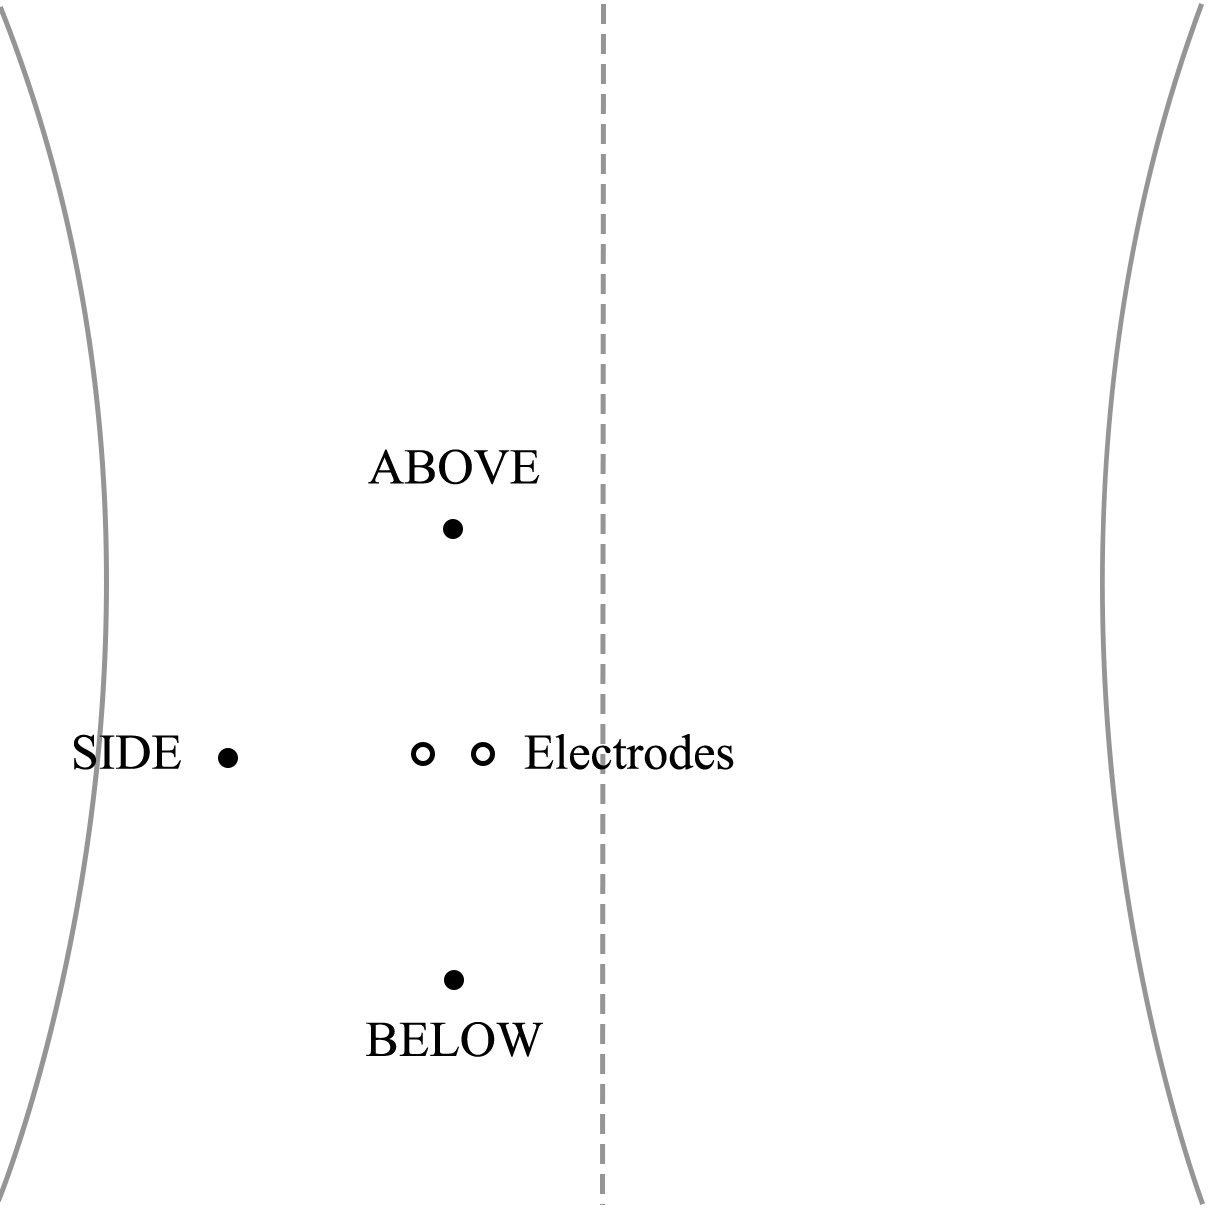
\includegraphics[width=\linewidth]{media/Other,+Figure+1.png}
\end{fullwidth}
\begin{adjustwidth}{-.5\fullwidthlen}{}
\caption{\emph{Arrangement of Tactors and Electrodes on the Back \parencite[][Adapted from]{Traxler2019}}}
\label{fig:fig4}
\end{adjustwidth}
\vskip3.7\baselineskip
\end{figure}
\subsection{Laboratory Setup}

The participants receive two types of stimuli at the same time, replicating the procedure in Traxler et al. \parencite{Traxler2019}. Stimulus onset and timing are controlled using Affect 4.0 \parencite{Spruyt2009}. A vibrotactile stimulus is delivered to the skin using tactors manufactured by Dancer Design taped to the participant's skin \parencite{Dancer Design0}. This stimulus is of fixed duration and a clearly perceptible intensity. Three tactors are used in the arrangement as the source of a CS (see Figure 1). The SIDE tactor is allocated to CS\textsubscript{neutral}, whereas the ABOVE and BELOW tactors are assigned to CS+ and CS- in a counterbalanced way across participants.




An electrocutaneous stimulation is delivered by passing a current across two surface electrodes located at the midpoint between the tactors to serve as the US (Figure 1). The current is delivered using a DS7A constant current stimulator \parencite{Digitimer Limited0}. The stimulation intensity is calibrated individually. The number of pulses delivered on each stimulation occasion is varied to provide a US\textsubscript{high} that is usually painful, a US\textsubscript{low} that is usually non-painful, and a US\textsubscript{test} that is calibrated to lie close to the pain threshold, the boundary between non-painful and painful.

\subsection{Tactor and Electrode Preparation}

On arrival, participants are seated straddling a chair in front of a desk with a computer monitor, mouse, and keyboard. Participants are asked to bend backwards to identify the point at which the greatest bend is seen. A point in the upper lumbar region is marked on the back, 2cm to the left of the spine, where the electrodes are placed such that the mark lies exactly between them. Three other points—4cm above, below, and to the left side of the electrodes—are marked, and the tactors are taped in place such that the closest border of each tactor lies at a tactor mark (Figure 1). Calibration is performed by the procedure described in Traxler et al. \parencite{Traxler2019}, with the CS\textsubscript{neutral} paired with each electrocutaneous stimulus. The CS\textsubscript{neutral} is used to provide vibratory stimulation consistent with the CS+/CS- stimuli that are later presented in the experimental trials to ensure that any modulation of pain by the vibration itself is consistent across calibration and experimental trials. Ratings of CS\textsubscript{neutral} trials from the experimental phase are not relevant to the research question and are therefore not analyzed.

\subsection{Experimental Trials}

Based on the experimental setup discussed previously, and given the pairing of CSs and USs, the experiment for a participant can theoretically consist of five different types of trials:

Training trials: Each training trial consists of one CS, with each of the three CS types used in different trials. There is no electrocutaneous stimulation (i.e., US) presented. These trials are conducted to familiarize the participants with the locations of the CS tactors. 

Baseline trials: The baseline trials consist of two combinations of stimulations: a CS+ with a simultaneous US\textsubscript{test} and a CS- with a simultaneous US\textsubscript{test}. These trials are used to record baseline pain ratings of participants before they are conditioned to associate the painful US with a particular CS.

Acquisition or learning trials: These trials consist of two combinations of stimulations: a CS+ with an US\textsubscript{high} and a CS- with an US\textsubscript{low}, and are meant to condition participants to associate painful US to CS+ and vice versa.

Test trials: These trials are the same as the two baseline trials: a CS+ with an US\textsubscript{test} and a CS- with an US\textsubscript{test}, and are meant to record pain ratings of participants to test whether they have associated the painful US with CS+ and vice versa.

Irrelevant trials: These trials consist of a CS\textsubscript{neutral} combined with an US\textsubscript{test} stimuli. These trials are noninformative and are included to satisfy the assumptions of the analytical approach; they are included only to achieve consistency in the time gaps between baseline or test trials. 

\subsection{Observed Variables}

The participants are requested to provide two reports on each trial. First, they rate the stimulation event on the Sensation and Pain Rating Scale \parencite[][SPARS; previously known as FESTNRS;]{Madden2017, Madden2019}. The SPARS is anchored at -50 (no sensation), 0 (the exact point at which the feeling transitions to pain), and 50 (worst pain imaginable). The two distinct ranges for non-painful (-50 to -1) and painful (1 to 50) are clearly marked and explained to the participants. Participants are explicitly advised to make an initial decision about whether a trial was non-painful or painful before assigning a rating from the appropriate side of the scale, without selecting 0 on SPARS. 

Second, the participant indicates the location at which they feel the vibrotactile stimulus from the three options “ABOVE”, “BELOW”, and “SIDE”. This is only used to confirm that the participants are identifying the location of the stimuli correctly. Given that discrimination of the vibrotactile stimuli is necessary for differential learning, participants who fail to identify the location of the stimulus correctly in at least 75\% of the trials are excluded and replaced by additional participants.

\subsection{Effect Size Measure and Test Statistic}

We are interested in calculating whether the participants judged trials of CS+/ US\textsubscript{test} and CS-/ US\textsubscript{test} as painful or non-painful differently for baseline and test trials. For this purpose, we first convert the SPARS ratings to a binary variable: 0 for non-painful (-50 to -1 on SPARS) and 1 for painful (1 to 50 on SPARS). A rating of 0 on SPARS can neither be classified as painful nor as non-painful, therefore these are considered indeterminate and were marked as missing. Then, we pair two trials, a CS+/ US\textsubscript{test} and a CS-/ US\textsubscript{test} and calculate the difference between the corresponding binary variables. The resulting difference indicates whether the participant is rating CS+/ US\textsubscript{test} and CS-/ US\textsubscript{test} differently. The difference can result in three different values: 1 when the CS+/ US\textsubscript{test} trial is rated as painful while the corresponding CS-/ US\textsubscript{test} trial is rated as non-painful; -1 when the CS+/ US\textsubscript{test} trial is rated as non-painful while the corresponding CS-/ US\textsubscript{test} trial is rated as painful; and finally, 0 when both CS+/ US\textsubscript{test} and CS-/ US\textsubscript{test} trials are rated as painful or both are rated as non-painful. This difference value, calculated from a pair of trials, constitutes one measurement in our SCE. A simple mean difference (MD) effect size measure is calculated as the difference between the means of the difference values derived from the test trial pairs and the difference values derived from the baseline trial pairs. Due to the flexibility of RTs, this effect size measure can also be used as the test statistic \parencite{Heyvaert2014a}. 

\subsection{Single-Case Design }

In this section, we describe our considerations regarding which SCE design to use in our experiment. We discuss several initial design possibilities that were chosen by trial and error and conclude with a final design.

\subsubsection{Initial Design Options}

Randomized Block Design. Since each of our measurements requires a pair of trials, we immediately considered a randomized block design (RBD) for the experiment. In an RBD SCE, similar to an RBD in traditional group designs, the measurement occasions are divided into small blocks, with each block containing administrations of all treatment conditions \parencite{Onghena2005}. For our study, a possible block consists of the two baseline (or test) trials, a CS+/ US\textsubscript{test} and a CS-/ US\textsubscript{test}, in random order. Hence, the experiment for a participant can consist of several blocks of baseline trial pairs, followed by a period of acquisition trials to condition the participants, followed by several blocks of test trial pairs. However, this design is immediately rejected, as an RBD SCE requires all treatment conditions to be applied inside a block. Since the effects of conditioning are acquired over a period of time and are expected to carry over to future trials, true alternation of treatment conditions is not possible in this experiment. 

AB Phase Design with In-Phase Acquisition. When we rejected the RBD, we realized that the experiment should consist of periods of baseline trial pairs and periods of test trial pairs. The simplest method to achieve this is using an AB phase design, with an A phase as the baseline condition and a subsequent B phase as the test condition \parencite{Barlow2009}. In favor of internal validity, the phase transition is preferably randomized. Each phase consists of several blocks of trials, each of which yields one measurement. Each measurement block in the baseline phase consists of \emph{k} irrelevant trial pairs (two CS\textsubscript{neutral}/ US\textsubscript{test}) and a baseline trial pair (a CS+/ US\textsubscript{test} and a CS-/ US\textsubscript{test} in random order). Similarly, each measurement block in the test phase consists of \emph{k} acquisition trial pairs (a CS+/ US\textsubscript{high} and a CS-/ US\textsubscript{low} in random order) followed by a test trial pair (a CS+/ US\textsubscript{test} and a CS-/ US\textsubscript{test} in random order). The number of irrelevant or acquisition trial pairs in each block, or \emph{k}, is set based on the required level of acquisition. A lower \emph{k} would mean we would need a lower number of trials to achieve a certain number of measurements, but would also typically result in weaker acquisition of associations, and vice versa for a higher \emph{k}. Unfortunately, this design has low acquisition of the associations as there is no learning period. Additionally, RTs for AB phase designs require a large number of measurements to achieve sufficient statistical power \parencite{Michiels2019, Ferron1995}. As a result, the experiment for a participant would need a very large number of trials over a significantly long time to ensure both high acquisition and enough measurements. As a result, this design is rejected in favor of a slightly modified AB phase design. A similar ABAB phase design is also rejected due to the potentially large number of trials required and possibility of carry-over effects between phases. 

\subsubsection{Final Design}

The final design combines elements from both previous designs: an AB phase design with both out-of-phase and in-phase learning. The baseline phase for this design contains several pairs of baseline trial pairs (a CS+/ US\textsubscript{test} and a CS-/ US\textsubscript{test} in random order), followed by a period of learning with only acquisition trial pairs (a CS+/ US\textsubscript{high} and a CS-/ US\textsubscript{low} in random order). Finally, the test phase includes test trial pairs (a CS+/ US\textsubscript{test} and a CS-/ US\textsubscript{test} in random order) with a few acquisition trial pairs in between at regular intervals to reinforce the associations and hence prevent extinction. The time of onset of the test phase is randomized. The experiment starts with a few training trials before the baseline phase. 

The number of trials and the number of participants are to be decided based on a power study and some pilot experiments. However, the guidelines for phase designs by Kratochwill et al. \parencite{Kratochwill2010a} recommend at least five measurements in both baseline and test phases. Since we are also curious about any increase or decrease in acquisition over time, we decide to include at least 15 measurements in the test phase. 

Due to the use of specialized equipment and individual calibration, multiple participants cannot be tested at the same time. Hence, simultaneous replication using a multiple baseline design (MBD), which is able to control for environmental confounding factors, is not possible \parencite{Barlow2009, Kazdin2011}. Instead, the experiment is to be run as a sequentially replicated AB phase design experiment. 

\subsection{Randomization Scheme and RT}

The design is randomized using intervention start point randomization for each participant \parencite{Edgington1975}. In this scheme, the total number of measurements and the minimum number of measurements in each phase is decided beforehand, and the intervention can start at any time point that satisfies these restrictions. Therefore, if the number of measurements is \emph{N}, and the minimum number of measurements in A and B phase are \emph{a} and \emph{b} respectively, the number of possible randomizations is \emph{r} = \emph{N} -- \emph{a} -- \emph{b} + 1. For \emph{P} participants with the same randomization scheme, the total number of randomizations for the replicated experiment is \emph{r}\textsuperscript{\emph{P}}. 

We conduct a single RT for all participants combined based on these \emph{r}\textsuperscript{\emph{P}} randomizations. The null hypothesis for this RT is that no difference exists between the baseline phase measurements and test phase measurements for all participants. As discussed previously, the measurements represent whether participants rate CS+/ US\textsubscript{test} trials as painful more frequently than CS-/ US\textsubscript{test} trials. Since the Pavlovian conditioning procedure is aimed at participants perceiving the CS+/ US\textsubscript{test} as more painful, the RT is one-sided with the alternate hypothesis being that the test phase measurements are higher than the baseline phase measurements for at least one participant. This RT can be conducted with the average (across participants) of the MD effect size measure discussed previously as the combined test statistic.

We use the Shiny SCDA (Single-Case Data Analysis) web app for SCEs to randomize and analyze the experiment \parencite{De2020a}. Whereas this web app does not include an option for simultaneously replicated AB phase design, it does include an MBD option. The MBD option in Shiny SCDA uses the Koehler-Levin regulated randomization procedure \parencite{Levin2018}, which, when using an identical set of possible start points for all participants, is analogous to our randomization scheme. Hence, we can both randomly select test phase start points and run the RT in Shiny SCDA. Additionally, we can plot the observed data for visual analysis in Shiny SCDA. 

\subsection{Pilot Tests}

We ran several pilot tests to estimate possible effect sizes and to test possible design choices. We first tested nine participants under slight variations of our initial design choice. Later, after a simulated power study and adjustments to the design, we tested another four participants. We analyzed these four tests using visual analysis and an RT in Shiny SCDA. These four tests were, however, not randomized, and the test phase for all four participants started at the tenth measurement occasion. However, for the purposes of demonstration, we ignored the assumption of randomization. We will discuss the results from these pilot tests, and the final four tests in particular in the Results section. 

There were two important takeaways from the first nine pilot tests that were very useful for the design of the power study. First, the observed MD effect sizes were extremely small. The average effect size from the first nine tests was slightly negative at -0.037, with a maximum of 0.143 and a minimum of -0.400. Second, the pilot tests also revealed difficulties in running the experiment for more than 30-35 minutes for a participant. Considering each trial took around 15 seconds, this gave us a maximum of around 140 trials.
\begin{table}[t!]
 \begin{fullwidth}
\caption{Estimated Power Simulated Using Different Values for Effect Size, Number of Measurements, and Number of Participants.}
\begin{tabular}{@{}p{4\smallwidth} p{4\smallwidth} S  S  S  S  S @{}}
\toprule          
&    & \multicolumn{5}{c}{Effect size} \\ \cmidrule(l){3-7} 
\multirow{-2}{=}{{\scriptsize No. of measurements}} & {\multirow{-2}{=}{\scriptsize No. of   participants}} & 0.1     & 0.2      & 0.3      & 0.4       & 0.5       \\  \midrule

$25$                            & $10$            & 10.3      & 19.0     & 32.2     & 48.6    & 66.1      \\

& $20$                                                              & 13.4      & 29.3     & 51.4     & 74.4      & 90.0      \\ 
        & $30$                                                              & 16.4      & 38.8     & 66.1     & 87.9      & 97.7      \\
& $40$                                                              & 18.9      & 47.5     & 77.4     & 94.8      & 99.5      \\
& $50$             & 22.2      & 54.7     & 85.1     & 97.9      & 99.9      \\
$30$                                                            & $10$                                                              & 13.0      & 25.9     & 45.0     & 66.1      & 83.9      \\
& $20$                                                              & 17.9      & 42.0     & 70.6     & 90.8      & 98.5      \\
& $30$                                                              & 21.9      &54.9     & 86.0     & 97.9      & 99.9      \\
& $40$                                                             & 26.4      & 65.2     & 92.7     & 99.6      & 100.0     \\
& $50$                                                              & 30.0      & 73.4     & 96.6     & 99.9      & 100.0     \\
$35$                                                            & $10 $                                                             & 14.3      & 31.4    & 55.0     & 77.4      & 92.7      \\
& $20$                                                              & 21.0      & 51.4     & 81.0     & 96.6      & 99.7      \\
& $30$                                                              & 27.4      & 65.5     & 93.3     & 99.7      & 100.0     \\
& $40$                                                              & 32.8      & 77.1     & 97.5     & 99.9      & 100.0     \\
    & $50$                                                              & 37.4      & 84.7     & 99.1     & 100.0     & 100.0     \\
$40$      & $10$                 & 15.4      & 36.0     & 63.9     & 84.9      & 96.3      \\
& $20$                                                              & 23.6      & 58.1     & 88.4     & 98.6      & 100.0     \\
& $30$                                                             & 30.7      & 74.0     & 96.8     & 99.9      & 100.0     \\
& $40$                                                              & 37.0      & 84.6     & 99.2     & 100.0     & 100.0     \\
& $50$                                                              & 42.8      & 90.4     & 99.8     & 100.0     & 100.0  
\bottomrule
\end{tabular}
\end{fullwidth}

\end{table}
\subsection{Power Study}

To ensure sufficient statistical power for our RT, we needed to first estimate power for different values of number of measurements (\emph{N}) and number of participants (\emph{P}), and then choose sufficiently high values of \emph{N} and \emph{P} for the experiment. 

Ideally, we would want to select the maximum \emph{N} possible within the limits of how long an experiment can be reasonably run. This strategy presents us with two advantages. First, increasing \emph{N} should result in reduction in the variability of the estimate of effect size. Second, maximizing \emph{N} should allow us to achieve sufficient power with lower \emph{P}, which directly equates to lower cost for the experiment.

We used the Monte Carlo method used by Ferron and Onghena \parencite{Ferron1996} to estimate power. In this method, several datasets are simulated under a set of simulation conditions. The proportion of these simulated datasets in which the RT leads to a rejection of the null hypothesis gives an estimate of statistical power for the given set of simulation conditions. A simulation study of such complexity is both difficult to program and computationally intensive to execute. Fortunately, we were able to modify and repurpose R code used by De, Michiels, Tanious, et al. \parencite{De2020} for this study. 

\subsubsection{Simulation Conditions}

The following three simulation conditions were varied for this power study:

Effect size: Based on the low effect sizes observed in the pilot tests, we simulated MD effect sizes of 0.1, 0.2, 0.3, 0.4, and 0.5 for the simulated observed data.

Number of measurements: We decided on a minimum of five measurements in the baseline phase and a minimum of 15 measurements in the test phase. As a result, the experiment needs more than 20 measurements. However, from the pilot tests it was evident that an experiment with more than 140 trials (70 trial pairs) was not feasible. Considering around 30 trials are required for the training and learning periods, and a few more acquisition trails for reinforcement during test phase, it was difficult to have more than 40 measurements (80 trials). Hence, we used 25, 30, 35, and 40 measurements for simulated data. 

Number of participants: Since the pilot tests revealed a small effect size, and the number of measurements is also limited, to ensure high power we considered a large range of participant count at 10, 20, 30, 40, and 50. 





% Please add the following required packages to your document preamble:
% \usepackage{booktabs}
% \usepackage{multirow}
% \usepackage[table,xcdraw]{xcolor}
% If you use beamer only pass "xcolor=table" option, i.e. \documentclass[xcolor=table]{beamer}
\begin{figure}[t!]
\captionsetup{width=\dimexpr \linewidth+\fullwidthlen\relax}
\begin{fullwidth}
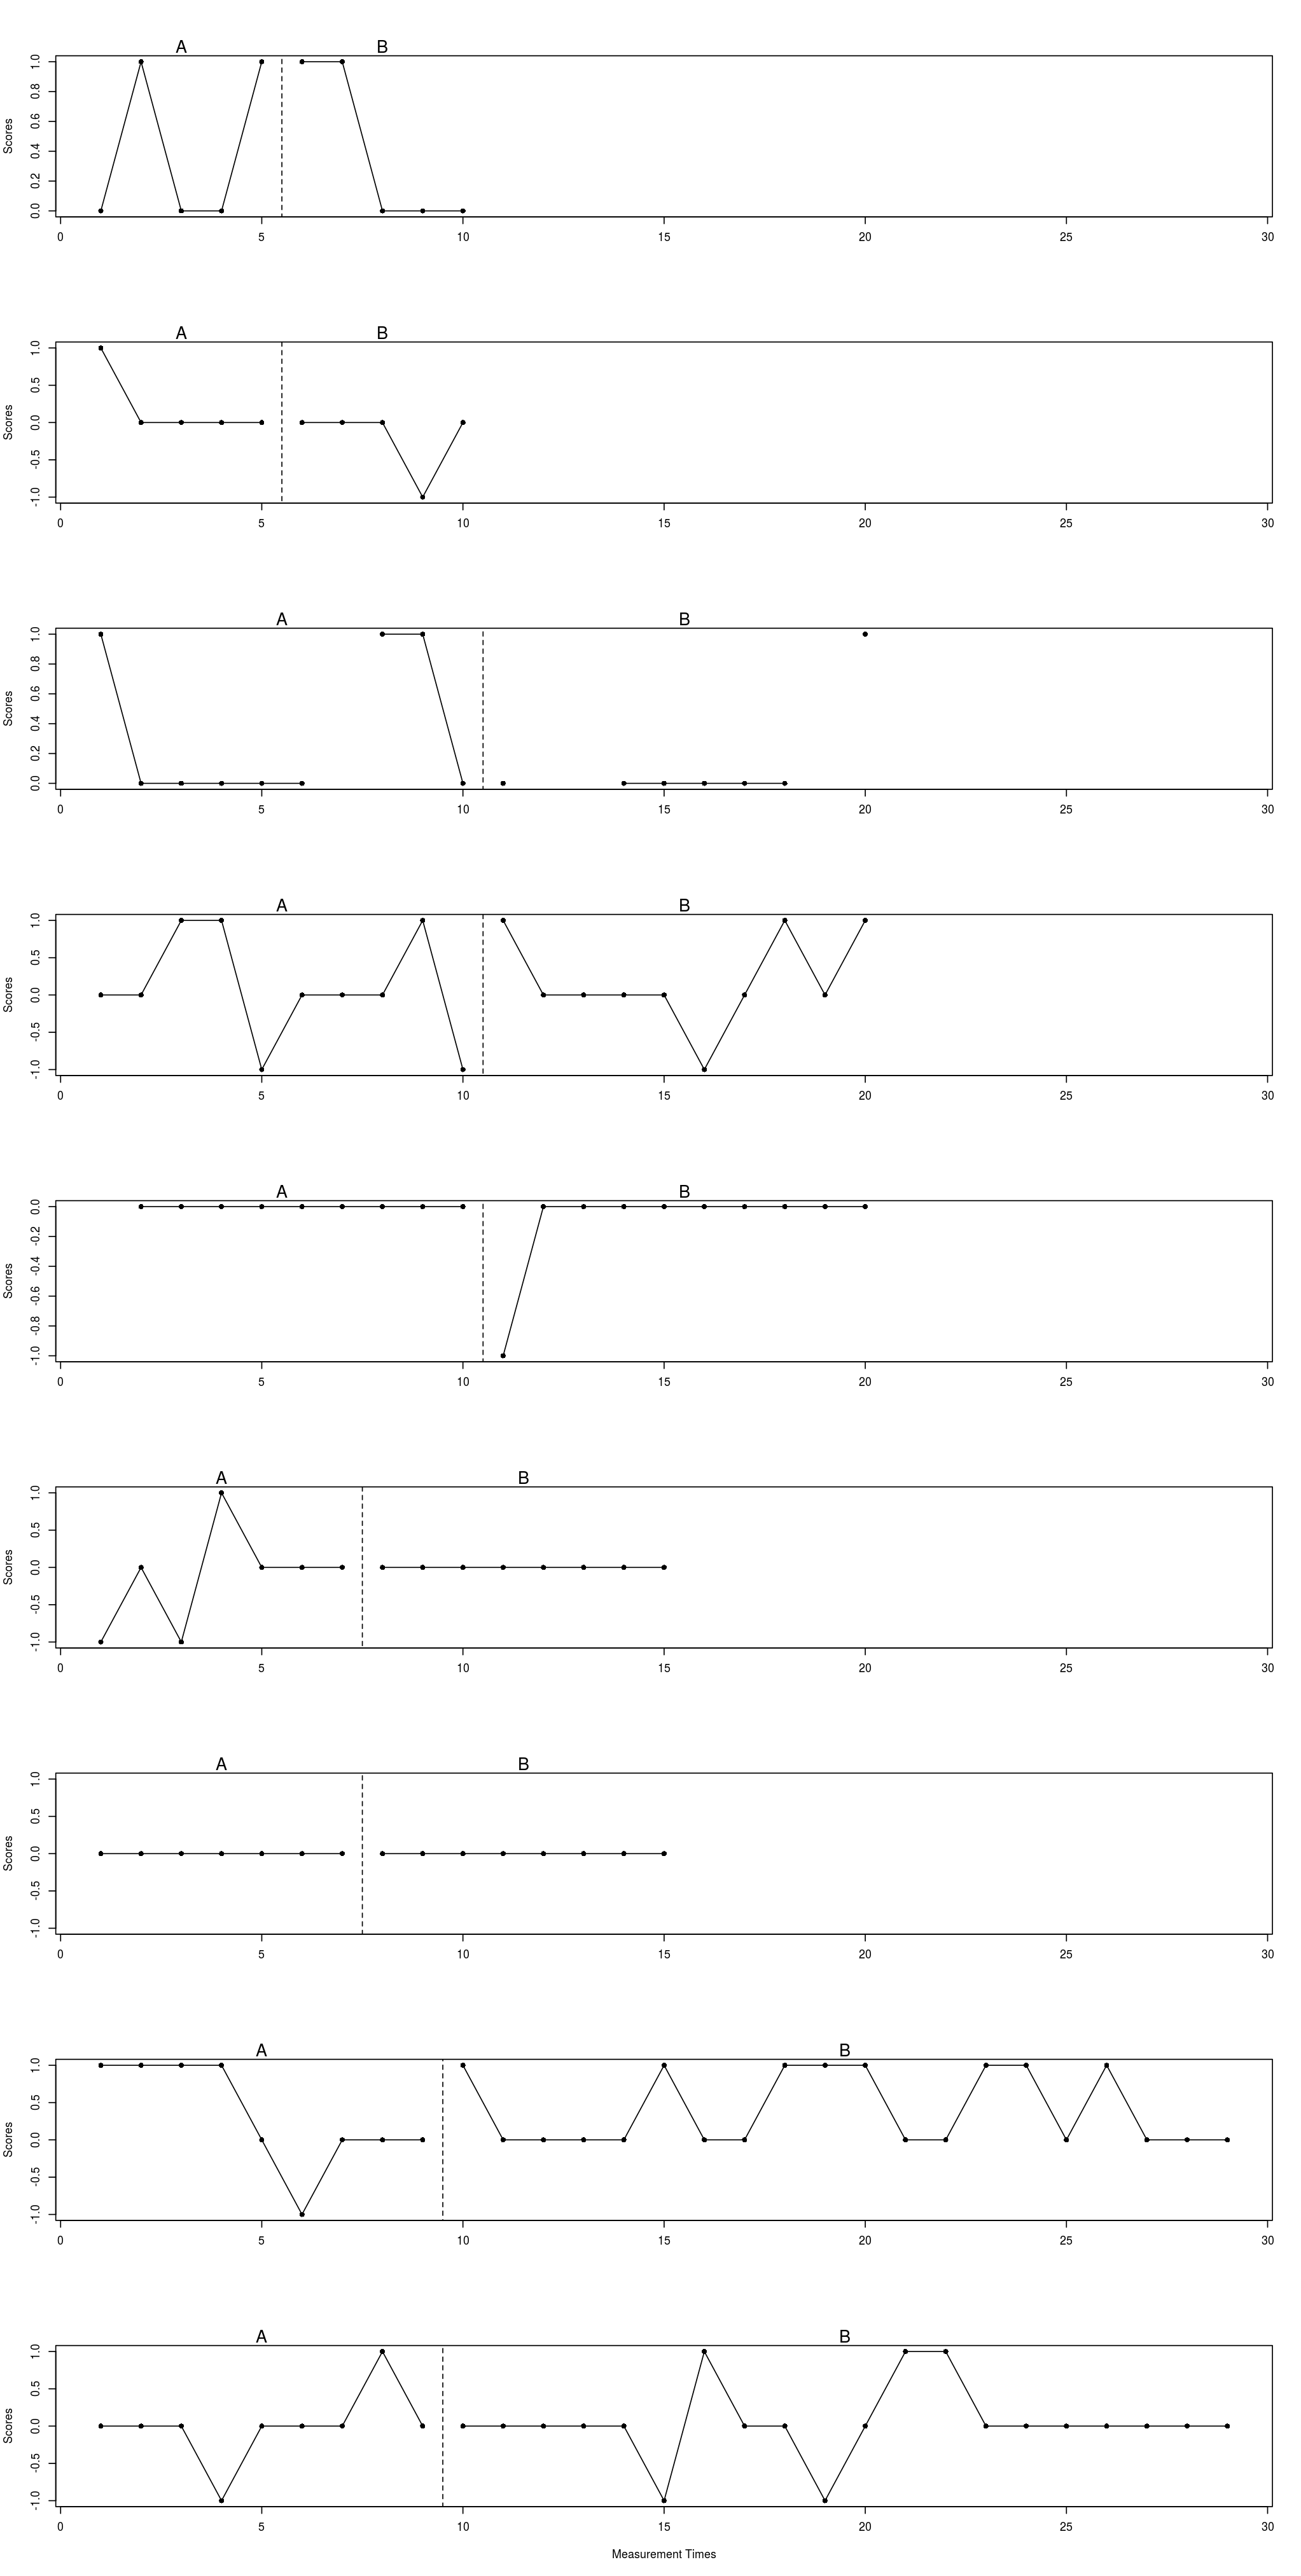
\includegraphics[width=\linewidth]{media/Other,+Figure+3.png}
\end{fullwidth}
\begin{adjustwidth}{-.5\fullwidthlen}{}
\caption{\emph{plot of ebserved scores obtained }\emph{from}\emph{ the initial nine participants in the pilot tests.}}
\label{fig:fig3}
\end{adjustwidth}
\end{figure}
\subsubsection{Other Simulation Parameters}

For the power study, we wanted to simulate observed values that were similar to the experiment. For the baseline, we assumed a symmetric distribution around 0 for the SPARS rating. Therefore, the painful/non-painful ratings were expected to be 0s and 1s equally for both CS+/ US\textsubscript{test} and CS-/ US\textsubscript{test} trials. Hence, an observed value corresponding to a trial pair in the baseline was expected to be 1 with 25\% probability, -1 with 25\% probability, and 0 with 50\% probability. We simulated observed values as 1, -1, and 0 with these probabilities. For the test phase, we increased the probability of 1 by half the selected effect size and decreased the probability of -1 by half the selected effect size. This resulted in an expected MD effect size equal to the selected effect size. 

Since the number of randomizations for the RT was huge, we simulated Monte Carlo RTs with 1000 randomizations \parencite{Edgington1969}. For estimating power, we simulated 10000 datasets for each set of simulation conditions. Finally, we used a 5\% level of significance for the simulated RTs.



The simulations were run on supercomputer nodes at the Flemish Supercomputer Center (Leuven, Belgium). This allowed testing more simulation conditions and achieve high accuracy simulating a large number of datasets for each simulation condition; however, the simulations can also be run at a smaller scale on a personal computer. 

\section{Results}

\subsection{Power Analysis}

The results from the power study (Table 1) revealed that due to the relatively small effect sizes and restricted number of measurements, the number of participants need to be high to achieve 80\% power. If we restrict the number of measurements to 30, which allows sufficient acquisition trials for learning and reinforcement within 30 minutes, 30 participants result in sufficient power even with a moderate effect size. 






Based on these results, we decided to run the final set of pilot tests with 30 measurements. We decided on six training trials (two trials for each type of CS) before the baseline phase, 24 acquisition trials between the baseline and test phases, and additionally one acquisition trial pair for reinforcement after two test trial pairs during the test phase. With a minimum of five measurements in the baseline phase, and a minimum of 15 measurements in the test phase, this design allows for 11 possible randomizations. Depending on the number of measurements in the test phase which will vary based on the test phase start point selected, the experiment could theoretically consist of 104 to 114 trials. This is the design we intend to follow in the final experiment with 30 participants (Figure 2).

\begin{figure}[t!]
\captionsetup{width=\dimexpr \linewidth+\fullwidthlen\relax}
\begin{fullwidth}
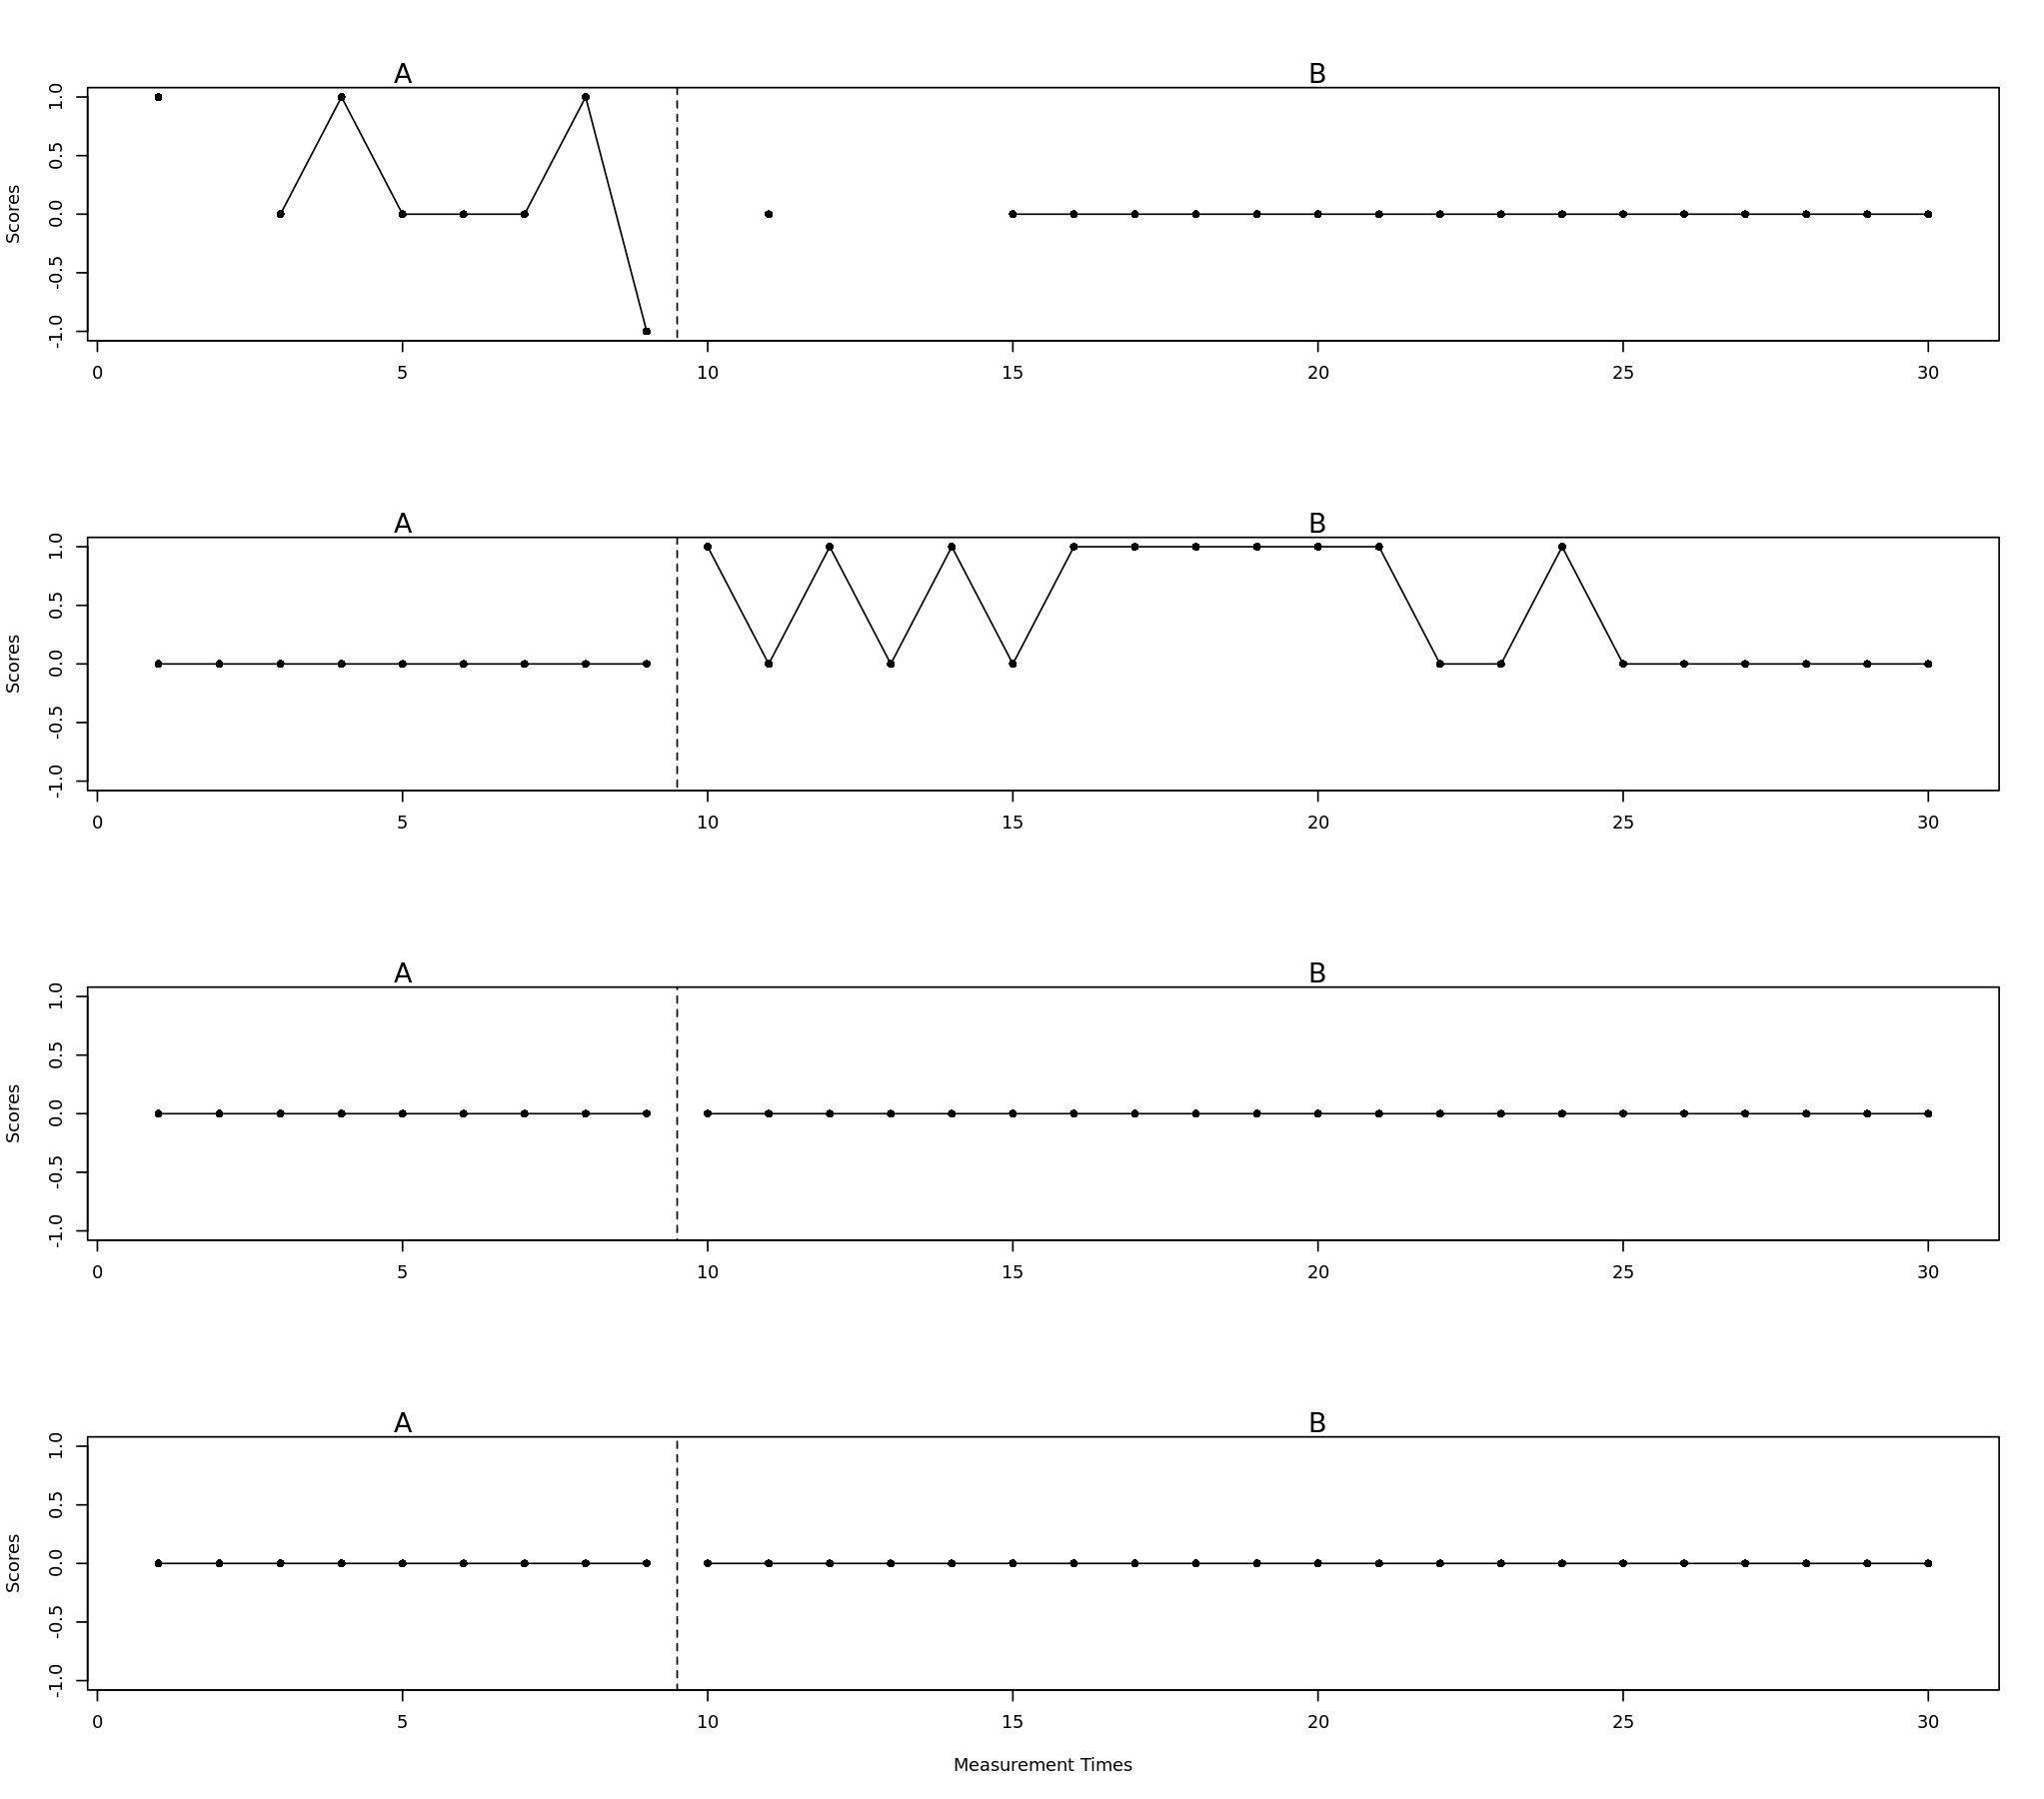
\includegraphics[width=\linewidth]{media/Other,+Figure+4.png}
\end{fullwidth}
\begin{adjustwidth}{-.5\fullwidthlen}{}
\caption{\emph{Plot of observed scores obtained }\emph{from}\emph{ the final four participants in the pilot tests.}}
\label{fig:fig4}
\end{adjustwidth}
\end{figure}
\subsection{Pilot Tests}

As mentioned previously, the initial nine pilot tests resulted in extremely small (and a few negative) effect sizes. The average MD effect size was -0.037, with a maximum of 0.143 and a minimum of -0.400. The low effect sizes indicated that the final design would need a large number of measurements and participants to achieve sufficient power in the RT. The first seven of these pilot tests consisted of 10-20 measurements each, which seemed too few. On the other hand, the last two pilot tests out of these consisted of 238 trials each. The feedback from both the experimenters and participants was that these tests were too long. These results influenced the decision to limit the number of trails to 140, remove irrelevant trial pairs from the baseline phase, and lower the number of acquisition trail pairs in the treatment phase. 




The later four pilot tests were run using the design parameters we decided on after the power study. The average MD effect size for these participants was 0.057, with a maximum of 0.476 and a minimum of -0.250. Visual analysis (Figure 4) revealed that the first, third, and fourth participant did not seem to show any sign of conditioning. However, the second participant seemed to show significant conditioning effects. This is also confirmed by the MD effect size for the second participant (0.476). Finally, a Monte Carlo RT with 1000 randomizations resulted in a \emph{p}-value of 0.112. Hence, the null hypothesis of the RT could not be rejected at a 5\% level of significance. 


\section{Discussion}


The power analysis and pilot test results confirm that the SCE design developed for this study can be effectively used to test the effect of classical conditioning on pain thresholds. The power study provides strong evidence that this design results in sufficient power if the number of measurements and participants are chosen correctly. The results from the final four pilot tests were encouraging. Even though the RT lacked power due to the small number of participants, the \emph{p}-value was low. The visual analysis also seemed to suggest a large effect for at least one participant. 

The final study using this protocol was not conducted immediately, due to lack of resources at the time. However, we hope to conduct this study as soon as the opportunity arises. Meanwhile, it seemed that the discussions regarding the SCE design and preparations for the study might be useful for other researchers developing similar protocols. Therefore, we decided to prepare this manuscript.

The final design suffers from a few limitations. The first limitation is the observed variable defined by us, which only yields values of -1, 0, and 1. Unfortunately, this restricts variation in observed data and can cause duplicates in the randomization distribution, which can affect power. An alternative is to use the difference between SPARS ratings from CS+/ US\textsubscript{test} and CS-/ US\textsubscript{test} trial pairs. However, this would require a slightly different hypothesis, which would not clarify whether classical conditioning can affect pain thresholds specifically.



The second limitation is due to the properties of the AB phase design. RTs using randomization of intervention start points in AB phase designs are known to lack power at lower sample sizes \parencite{Michiels2019}. AB phase designs do not satisfy the guidelines set by Kratochwill et al. \parencite{Kratochwill2010a} without multiple replications. Since we are not sure how quickly the effect of our conditioning is reversed, we cannot use phase designs with more phase changes, such as the ABAB phase design. Due to the requirement of specialized equipment, we cannot use an MBD. Critically, we cannot increase the number of measurements due to time constraints. Therefore, we have to rely on sequential replications for both validity and statistical power. 

The power study for this design also presents certain limitations. We used only one possible distribution of the SPARS ratings to simulate our observed data. While the assumption of a symmetric distribution around 0 is not unreasonable, with more pilot data, it might be possible to simulate using a distribution that resembles the observed data. We also did not account for any variability in effect size across participants. Instead, we simulated an equal effect size for all participants. However, we believe these are reasonable assumptions given the scope of our study. 

Finally, we conducted Monte Carlo RTs for both the power study and the pilot data. As discussed previously, the number of possible randomizations for this design is \emph{r}\textsuperscript{\emph{P}}, where \emph{r} denotes the number of possible randomizations for one participant, and \emph{P} denotes the number of participants. Even for the smaller scale of the pilot data, computing 11\textsuperscript{4} possible randomizations would have been extremely costly. Monte Carlo RTs present a simple alternative to this computation cost while maintaining sufficient statistical power \parencite{Edgington1969, Hope1968}. Hence, we intend to conduct a Monte Carlo RT in the final experiment.

As introduced earlier, this design presents certain advantages over traditional group study designs. Single-case designs are a better match for studying within-person changes, because they allow detailed insight into within-individual processes rather than assuming that the response of all individuals in a group is consistent. Additionally, these designs typically require a smaller number of participants. This allows for a lower overall cost and is particularly important for pain studies because it can be difficult to recruit participants.
Tamal Kumar De, Victoria J. Madden, Johan W. S. Vlaeyen, and Patrick Onghena

\section{Conclusion}

In this manuscript, we described how we used trial and error to design an SCE testing whether classical conditioning can affect pain thresholds. We used a sequentially replicated AB phase design and conducted a simulated power study to determine sample size. We decided on 30 participants and 30 measurements per participant. Finally, we ran some pilot tests using our design. While the results from the pilot tests were inconclusive, they were sufficiently encouraging that we plan to conduct the full study in the near future.

\begin{originalPurpose}

In this manuscript, our purpose is to describe how we used a trial and error approach to design a customized single-case experiment (SCE) to test the effect of classical conditioning on pain thresholds. We hope that this information helps readers who plan to implement an SCE in better understanding the steps involved and possible challenges. We wish to focus on using the flexible nature of SCEs to adapt to the requirements of the experiment. We also wish to highlight the necessity of exploring various available statistical methods and statistical power requirements for these methods prior to starting the experiment. Finally, we demonstrate how SCEs can serve as a viable avenue for pilot-testing new therapies and treatments at a small scale before implementing larger scale studies.
\end{originalPurpose}
\section{Funding}
This research is supported by the Asthenes long-term structural funding - Methusalem grant (nr. METH/15/011) by the Flemish Government, Belgium. The resources and services used in this work were provided by the VSC (Flemish Supercomputer Centre), funded by the Research Foundation - Flanders (FWO) and the Flemish Government. Research collaboration supported by the IASP Developing Countries Collaborative Research Grant. VJM is supported by the Fogarty International Center of the National Institutes of Health (award K43TW011442). The content is solely the responsibility of the authors and does not necessarily represent the official views of the National Institutes of Health.

\section{Data Availability}

The data and R code used in this study are openly available on \href{https://osf.io/d9mfn/?view\_only=6b9bd4580dbf42b4952e551972f48c68}{Open Science Foundation}  




\printbibliography

 \onecolumn
\n
\section{Appendix}


\begin{table}[t!]

  \caption{\emph{Observed scores for the initial nine pilot tests.}}
\label{tab:table2}
\begin{tabular}{c  c  c  c  c  c  c  c  c  c  c  c  c  c  c  c  c  c}
\toprule

  P1 & V1 & P2 & V2 & P3 & V3 & P4 & V4 & P5 & V5 & P6 & V6 & P7 & V7
  & P8 & V8 & P9 & V9\\ \midrule
A & 0 & A & 1 & A & 1 & A & 0 & A & NA & A & -1 & A & 0 & A & 1 & A & 0\\
A & 1 & A & 0 & A & 0 & A & 0 & A & 0 & A & 0 & A & 0 & A & 1 & A & 0\\
A & 0 & A & 0 & A & 0 & A & 1 & A & 0 & A & -1 & A & 0 & A & 1 & A & 0\\
A & 0 & A & 0 & A & 0 & A & 1 & A & 0 & A & 1 & A & 0 & A & 1 & A & -1\\
A & 1 & A & 0 & A & 0 & A & -1 & A & 0 & A & 0 & A & 0 & A & 0 & A & 0\\
B & 1 & B & 0 & A & 0 & A & 0 & A & 0 & A & 0 & A & 0 & A & -1 & A & 0\\
B & 1 & B & 0 & A & NA & A & 0 & A & 0 & A & 0 & A & 0 & A & 0 & A & 0\\
B & 0 & B & 0 & A & 1 & A & 0 & A & 0 & B & 0 & B & 0 & A & 0 & A & 1\\
B & 0 & B & -1 & A & 1 & A & 1 & A & 0 & B & 0 & B & 0 & A & 0 & A & 0\\
B & 0 & B & 0 & A & 0 & A & -1 & A & 0 & B & 0 & B & 0 & B & 1 & B & 0\\
  &   &   &   & B & 0 & B & 1 & B & -1 & B & 0 & B & 0 & B & 0 & B & 0\\
  &   &   &   & B & NA & B & 0 & B & 0 & B & 0 & B & 0 & B & 0 & B & 0\\
  &   &   &   & B & NA & B & 0 & B & 0 & B & 0 & B & 0 & B & 0 & B & 0\\
  &   &   &   & B & 0 & B & 0 & B & 0 & B & 0 & B & 0 & B & 0 & B & 0\\
  &   &   &   & B & 0 & B & 0 & B & 0 & B & 0 & B & 0 & B & 1 & B & -1\\
  &   &   &   & B & 0 & B & -1 & B & 0 &   &   &   &   & B & 0 & B & 1\\
  &   &   &   & B & 0 & B & 0 & B & 0 &   &   &   &   & B & 0 & B & 0\\
  &   &   &   & B & 0 & B & 1 & B & 0 &   &   &   &   & B & 1 & B & 0\\
  &   &   &   & B & NA & B & 0 & B & 0 &   &   &   &   & B & 1 & B & -1\\
  &   &   &   & B & 1 & B & 1 & B & 0 &   &   &   &   & B & 1 & B & 0\\
  &   &   &   &   &   &   &   &   &   &   &   &   &   & B & 0 & B & 1\\
  &   &   &   &   &   &   &   &   &   &   &   &   &   & B & 0 & B & 1\\
  &   &   &   &   &   &   &   &   &   &   &   &   &   & B & 1 & B & 0\\
  &   &   &   &   &   &   &   &   &   &   &   &   &   & B & 1 & B & 0\\
  &   &   &   &   &   &   &   &   &   &   &   &   &   & B & 0 & B & 0\\
  &   &   &   &   &   &   &   &   &   &   &   &   &   & B & 1 & B & 0\\
  &   &   &   &   &   &   &   &   &   &   &   &   &   & B & 0 & B & 0\\
  &   &   &   &   &   &   &   &   &   &   &   &   &   & B & 0 & B & 0\\
  &   &   &   &   &   &   &   &   &   &   &   &   &   & B & 0 & B & 0\\
\bottomrule

\end{tabular}


\end{table}







\begin{table}[t]

  \caption{Observed scores from the final four pilot tests formatted for Shiny SCDA.}
  \label{tab:table3}
\begin{tabular}{c  c  c  c  c  c  c  c}
\toprule
  P10 & V10 & P11 & V11 & P12 & V12 & P13 & V13\\
  \midrule
A & 1 & A & 0 & A & 0 & A & 0\\
A & NA & A & 0 & A & 0 & A & 0\\
A & 0 & A & 0 & A & 0 & A & 0\\
A & 1 & A & 0 & A & 0 & A & 0\\
A & 0 & A & 0 & A & 0 & A & 0\\
A & 0 & A & 0 & A & 0 & A & 0\\
A & 0 & A & 0 & A & 0 & A & 0\\
A & 1 & A & 0 & A & 0 & A & 0\\
A & -1 & A & 0 & A & 0 & A & 0\\
B & NA & B & 1 & B & 0 & B & 0\\
B & 0 & B & 0 & B & 0 & B & 0\\
B & NA & B & 1 & B & 0 & B & 0\\
B & NA & B & 0 & B & 0 & B & 0\\
B & NA & B & 1 & B & 0 & B & 0\\
B & 0 & B & 0 & B & 0 & B & 0\\
B & 0 & B & 1 & B & 0 & B & 0\\
B & 0 & B & 1 & B & 0 & B & 0\\
B & 0 & B & 1 & B & 0 & B & 0\\
B & 0 & B & 1 & B & 0 & B & 0\\
B & 0 & B & 1 & B & 0 & B & 0\\
B & 0 & B & 1 & B & 0 & B & 0\\
B & 0 & B & 0 & B & 0 & B & 0\\
B & 0 & B & 0 & B & 0 & B & 0\\
B & 0 & B & 1 & B & 0 & B & 0\\
B & 0 & B & 0 & B & 0 & B & 0\\
B & 0 & B & 0 & B & 0 & B & 0\\
B & 0 & B & 0 & B & 0 & B & 0\\
B & 0 & B & 0 & B & 0 & B & 0\\
B & 0 & B & 0 & B & 0 & B & 0\\
B & 0 & B & 0 & B & 0 & B & 0\\
\bottomrule


\end{tabular}


\end{table}










\end{document}
